%\documentclass{acm-book-v2}
%\RequirePackage[errorshow]{tracefnt}
%\newcommand{\mpage}[1]{}
%%\newcommand{\indexfn}[1]{}

%%%\usepackage{showframe}

%\usepackage{custom-tooltip}
%\usepackage{custom-tooltip-Alt-Text-View}



%\begin{document}

\setcounter{chapter}{1}



\chapter{\label{chap:2}From Algorithms to Software}

This chapter clarifies how abstract algorithms can be transformed into software programs and how computers execute them. The main concepts and models introduced by Turing and von Neumann are explained in a simple way. Algorithms and software principles are compared, with an explanation of how these two concepts created new ways to address and solve problems.


\section{\label{sec:2.1}Hilbert, G\"{o}del, and Turing}
As discussed in the previous chapter, although eminent scientists and
mathematicians such as Wilhelm Schickard, Blaise Pascal, Gottfried
Wilhelm von \hbox{Leibniz,} and Charles Babbage had worked from the early 17th century onwards to design and implement machines capable of performing calculations automatically, the main contributions to the birth and development of the science of computers were provided in the early decades of the 20th century by Alan Turing and John von \hbox{Neumann.} They contributed, respectively, to the design of the abstract mathematical model of computers (the so-called \textit{Turing machine}) and the general architecture of electronic digital computers (\textit{von Neumann architecture}) that is the basis of most modern computers. However, before the fundamental work of Turing and von \hbox{Neumann,} the main occurrence that unwittingly stimulated the birth of \hbox{modern} computer science was the research project proposed in the early 1920s by the German mathematician and physicist David Hilbert that aimed at expanding the foundations of classical mathematics, which has come to be known as Hilbert's Program. Twenty years previously, at the 1900 International Congress of \hbox{Mathematicians} in Paris and in a subsequent publication, Hilbert presented a list of 23 unsolved mathematical problems. This list has been recognized as the most important compilation of open problems ever to be proposed by an individual mathematician. Some of the problems were\vadjust{\vspace*{12pt}\pagebreak} solved within a short time after the Hilbert formulation. Others were discussed by several logicians and mathematicians throughout the following 20 years.

Due to the paramount importance of the formulated problems, Hilbert called for a formalization program of all of mathematics in an axiomatic form, together with a proof that the axiomatization of mathematics is consistent. He was positive about the solution of the problems as he was thinking that every mathematical problem should have a solution even if that solution was a proof that the original problem is impossible to solve. Famously, he believed that we could always know this because, as he said during his address to the International Congress of Mathematicians in Paris, ``in mathematics there is no ignorabimus.'' Work on the program progressed significantly in the 1920s with contributions from logicians such as Paul Bernays, Wilhelm Ackermann, John von Neumann, and Jacques Herbrand. The program also had a great influence on Kurt G\"{o}del, whose work on the incompleteness theorems was motivated by Hilbert's Program. In fact, the second problem in Hilbert's list called for a proof that the arithmetic of real numbers is consistent, that is, it is free of any internal contradictions. When G\"{o}del started studying this problem, other mathematicians such as von Neumann and \hbox{Ackermann} seemed to be very close to completing a formal proof of the consistency of Peano's arithmetic. G\"{o}del himself was confident of being able to prove the consistency of more general systems relative to Peano's arithmetic, thereby helping to solve the second Hilbert problem. Contrary to his expectations, G\"{o}del did not prove the consistency of the arithmetic. Moreover, he proved that it was formally impossible to demonstrate that the arithmetic of real numbers is consistent.

The G\"{o}del result was one of the most significant in modern logic and in general set the limits of formal systems. In a strange twist of fate, G\"{o}del delivered his results in September 1930 in K\"{o}nigsberg just one day before Hilbert's address to the Society of German Scientists and Physicians in the same city. There, Hilbert expressed again his positive wish: ``We must not believe those, who today, with philosophical bearing and deliberative tone, prophesy the fall of culture and accept the ignorabimus. For us there is no ignorabimus, and in my opinion none whatever in natural science. In opposition to the foolish ignorabimus our slogan shall be `We must know, we will know'.'' [\citealt{chap:02:Smith:2014}]. Hilbert obviously had not yet known that based on G\"{o}del's results his goals of finding a complete and consistent set of axioms for all mathematics had the day before been proven to be unattainable.

Two months later, in November 1930, G\"{o}del submitted a paper to be published in the 1931 volume of \textit{Monatshefte f\"{u}r Mathematik und Physik} titled ``On formally undecidable propositions of principia mathematica and related systems I'' [\citealt{chap:02:Godel:1931}], presenting his two theorems of incompleteness as theorems VI and XI, respectively. Unlike Hilbert, von Neumann, who was in the audience during G\"{o}del's speech in K\"{o}nigsberg and was at the time working on similar problems, immediately understood the great importance of that result. In fact, on November 20, von Neumann wrote a letter to G\"{o}del regarding a ``remarkable'' corollary of G\"{o}del's result he had just discovered. It was about the unprovability of consistency (the so-called ``Theorem~XI''). G\"{o}del himself, however, had found the same idea and at that time had already sent for publication the final version of his article that also contained the second incompleteness theorem. Some sources reported the John von Neumann decided to stop his studies on logic after learning about the results achieved by G\"{o}del. Some years later, he said: ``Kurt G\"{o}del's achievement in \hbox{modern} logic is singular and monumental---indeed it is more than a monument, it is a landmark which will remain visible far in space and time.''



G\"{o}del's incompleteness theorems show that for any formal axiomatic system (a system of axioms equipped with rules of inference that allow one to generate new theorems) satisfying certain minimal requirements, there exist questions that cannot be answered within that system. In particular, Theorem VI states that no consistent system of axioms \textit{F} whose theorems can be expressed by an effective procedure, that is, an algorithm, is complete, that is, capable of proving all truths about the arithmetic of natural numbers. This means that for any such consistent formal system, there will always be statements about natural numbers that are true but which are unprovable within the same system. More exactly, the first incompleteness theorem shows that in any formal system \textit{F} sufficiently expressive to contain arithmetic, there is one formula \textit{f} such that, if \textit{F} is coherent, then neither \textit{f} nor its negation \textit{not-f} are demonstrable in \textit{F}. Therefore, logical consistency and completeness are incompatible. The second incompleteness theorem (Theorem~XI) is an extension of the first, showing that such a formal system \textit{F} (for instance, Peano's arithmetic) cannot demonstrate its own consistency. Logicians and mathematicians generally believe that G\"{o}del's incompleteness theorems dealt a decisive blow to Hilbert's second problem that asked for a finitary consistency proof for arithmetic. In fact, the second incompleteness theorem is often viewed as making that problem impossible. As a general consequence, the two theorems show that Hilbert's program that aimed to find a complete and consistent set of axioms for all mathematics is impossible.

The incompleteness theorems proved by G\"{o}del were the first and the most important theorems on the limitations of formal systems. Just two years later in 1933, Alfred Tarski proved the so-called ``undefinability theorem'' dealing with the formal undefinability of truth. Tarski's theorem states that arithmetical truth cannot be defined within arithmetic itself. Informally, this means that truth of the language of a formal system must be undefinable in the system. After this result, two other contributions by Alonso Church and Alan Turing proved the\break limits of Hilbert's program and contributed to the foundation of computer science. In the framework of his program, presented at the 1928 International Congress of Mathematicians in Bologna, Italy, Hilbert posed a problem that became known as \textit{Entscheidungsproblem} (decision problem). That problem asks for an algorithm that considers, as input, a statement, and answers ``Yes'' or ``No'' [\citealt{chap:02:Turing:1937}] to whether the statement is valid in every structure satisfying the axioms, that is, it is universally valid. Indeed, the \textit{Entscheidungsproblem} could be solved by an algorithm (a mechanical procedure) capable of deciding whether any given statement is provable from the axioms using the rules of logic. Seven years later, between 1935 and 1936, Alan Turing and Alonzo Church independently proved that a general solution to the \textit{Entscheidungsproblem} is not possible. In their works, it is assumed that the intuitive notion of ``effectively calculable,'' that is, computable through a mechanical method, is captured by the functions computable by a Turing machine or, equivalently, by those expressible in a formalism known as \textit{lambda calculus}.\footnote{Lambda calculus ($\lambda$\textit{-calculus}) is a universal formal model of computation allowing for expressing algorithms based on function abstraction and application using variable binding and \hbox{substitution.} For example, $\lambda x.x$ represents the identity function $f(x)=x$, whereas the function $\lambda x.x{}^{2}+1$ represents the function $f(x)=x^{2}+1$. Church proved that every expression of lambda calculus corresponds to a well-defined computational procedure (algorithm), thus giving a rigorous definition of effective computability (computable function) as requested by Hilbert.} The American mathematician and logician Church proved that Hilbert's \textit{Entscheidungsproblem} is unsolvable, and Turing's theorem states that there is no algorithm to solve the halting problem.

In fact, to be able to respond to Hilbert's decision problem in a rigorous way, it was necessary to specify in a formal manner the concept of an algorithm. Alonzo Church, with the contribution of his student Stephen Kleene, proposed the lambda calculus, while Alan Turing proposed the abstract machines theoretical model (now known as ``Turing machines''). In the spring of 1935, Turing was in \hbox{Cambridge} to attend a course of lectures on the foundations of mathematics taught by the brilliant mathematician Max Newman [\citealt{chap:02:Davis:2012}]. In one of the lectures, Turing learned of the \textit{Entscheidungsproblem} proposed by Hilbert in 1928. After that lecture, Turing began to wonder how it could prove that a similar algorithm (i.e., a mechanical procedure) did not exist. In about a year, he succeeded in this objective and in doing so he defined a mathematical model of an abstract computing device. This result was achieved in the spring of 1936, two years after completing his undergraduate degree, when Turing introduced the concept of the ``Turing machine'' in the paper titled ``On computable numbers, with an application to the Entscheidungsproblem'' that he submitted in May 1936 and was accepted in November 1936 [\citealt{chap:02:Turing:1937}]. This model has since become the main abstract model of computation used by computer scientists.

In that paper, Turing replaced G\"{o}del's universal arithmetic-based formal language with the abstract and simple theoretical devices that became known as Turing machines. In this way, he reframed G\"{o}del's results on the limits of proof and computation, proving that his ``universal computing machine'' would be capable of performing any possible mathematical computation if it were representable as an algorithm. From this, he deduced that if a computation problem cannot be expressed as an algorithm, that is, cannot be executed by a Turing machine, then there is no solution for that problem. According to Turing's definition, a \textit{computing machine} is a machine capable of a finite set of configurations $q_{1},\ldots ,q_{n}$ (the so-called \textit{m}-configurations). Formally, a Turing machine is defined as a quadruple $T = (Q, \Sigma , s, \delta )$ where:

\begin{itemize}
\item \textit{Q} is a finite set of states \textit{q},

\item $\Sigma $ is a finite set of symbols,

\item \textit{q} is the initial state $q\in Q$, and

\item $\delta$ is a transition function determining the next move as follows:
\begin{equation*}
\delta :(Q \times \Sigma )\to (\Sigma  \times  \{ L,\ R\}  \times Q).
\end{equation*}
\end{itemize}

\noindent To give a more realistic representation of his computing machine, Turing described it as an abstract machine that is supplied with

\begin{itemize}
\item A one-way infinite and one-dimensional tape divided into squares each capable of carrying exactly one symbol. The tape is assumed to be arbitrarily extendable to the left and to the right to have as much tape as it needs for computation.

\item A head that can read and write symbols on the tape and move the tape left and right one cell at a time.

\item A state register that stores the state of the machine, one of finitely many, and including a special start state with which the state register is initialized. In Turing's intention, the value of this register corresponds to the ``state of mind'' of a person performing the computations.

\item A finite table of instructions that, given the machine state $q_{i}$ and the current symbol $\underline{s}_{j}$ it is reading on the tape, tells the machine to execute the following in sequence steps:
\begin{enumerate}
\item[(1)] Either erase or write a symbol, replacing $\underline{s}_{j}$ with $s_{i,j}$.

\item[(2)] Move the head one step left or one step right or stay in the same position.

\item[(3)] Stay in the same or go to a new state as prescribed $q_{i,j}$.
\end{enumerate}
\end{itemize}

\noindent Turing went on to prove that there was no general solution to the decision problem (\textit{Entscheidungsproblem}) by showing that it is not possible to decide algorithmically whether, for all possible algorithm--input pairs, a Turing machine will ever halt or continue to compute forever (i.e., the halting problem for Turing machines is undecidable). The halting problem was then the way in which Turing gave an answer to the Hilbert's decision problem proving that mathematics is undecidable. That problem is also very important because it was one of the first problems to be proved undecidable. It is worth noting that in his paper Turing's main aim was to define computability, not algorithms. His paper argued that every function on natural numbers that can be computed by a (human or automatic) computer can also be computed by a Turing machine. As mentioned previously, the Turing machine abstraction, while it served to solve the decision problem, also became the main model of computability used by computer scientists for studying algorithm design and complexity and for building real computers. This is because the abstract notion of Turing's computing machine captures \textit{all} computable \hbox{problems} (as stated by the so-called \textit{Church--Turing thesis}). This implies also that any problem not computable by a Turing machine is not computable by whatever means.

\section{\label{sec:2.2}John von Neumann and the EDVAC}

As introduced in Chapter~\ExternalLink{chap:1}{1}, just after the historical results achieved by Alonzo Church and Alan Turing and the definition of the abstract universal computing machine by Turing, from late 1935 to the mid-1940s a few practical computing machines were designed and built. Some of these designers often worked ignoring the projects of others. Some of the new computers were built using electromechanical relays for their circuits while others exploited vacuum tube technology. In 1935, Howard H. Aiken considered building an automated computing machine originally called the Automatic Sequence Controlled Calculator (ASCC) and later the Harvard Mark I, whose construction was completed in 1943. While Aiken was working on the ACSS computer, Konrad Zuse in Germany exploited the Turing concepts to implement his Z3 computer, and John Atanasoff with the help of his student Clifford Berry developed the Atanasoff--Berry Computer (ABC) digital computing machine whose design inspired the project led by J. Presper Eckert and John Mauchly for implementing the Electronic Numerical Integrator and Computer (ENIAC).

The ENIAC project started in the summer of 1943, during World War II, and was completed in December 1945. The ENIAC machine was funded by the United States Army, and its construction was announced to the public in February 1946. The machine was used for about ten years. The ENIAC was utilized for military purposes, for instance, the calculation of artillery trajectories. It was also used for implementing a very simplified mathematical model of the H-bomb explosion. That computer was capable of approximately 5,000 calculations per second and in computing projectile trajectories it usually took a few tens of seconds, while for the same task a human specialist on average employed around 20 hours. However, it must be noted that the task of studying a problem and coding it onto the computer was difficult at that time---it typically took a few weeks. We should also consider that ENIAC was not a computer that stored the sequences of instructions in an electronically or optically accessible memory; it was only a large collection of arithmetic machines that originally had algorithms set up into the computer by a combination of plugboard wiring and three portable function tables. For this reason, after the algorithm was defined and its operational steps written on paper, the procedure of getting the code into the machine by manipulating its switches and cables could take a few days.

John von Neumann was aware of the ENIAC's development while working at the Los Alamos National Laboratory, and he joined the ENIAC team in 1944 upon the invitation of mathematician Herman Goldstine. At that time, the ENIAC creators John Mauchly and J. Presper Eckert had already proposed the construction of ENIAC's successor called the Electronic Discrete Variable Automatic Computer (EDVAC). Von Neumann joined Eckert and Mauchly in designing the EDVAC, and, in particular, he worked on the design of the logic functioning of the new computer. During his work on the logic design of EDVAC, von Neumann wrote his well-known \textit{First Draft of a Report on the EDVAC} [\citealt{chap:02:Neumann:1945}], which contains the first published description of the logical design of a computer using the stored-program concept, which has come to be known as the ``von Neumann architecture'' whose roots are in the Turing papers on the universal computing machine [\citealt{chap:02:Turing:1937}]. In contrast to ENIAC's decimal representation, data in the EDVAC were represented in binary notation and its architecture included a memory unit that stored both program data and instructions.

Von Neumann's \textit{First Draft} did not focus on mathematical logic and theorems; it described the basic components of the architecture of an actual computer and the technologies by which it could be implemented. At the same time, von Neumann's proposal did abstract away from details of the hardware to be used. The incomplete document reviewed discussions among the team working on ENIAC and its successor. The first page of the \textit{First Draft} cites only von Neumann as author; \hbox{however,} some on the EDVAC design team, including Eckert and Mauchly, argued that the stored-program concept, that is, much of the work represented in the \textit{Draft}, had evolved out of meetings at the University of Pennsylvania's Moore School of Electrical Engineering, not from the solitary work of von Neumann. Regardless of how the events really unfolded, the von Neumann architecture was used to implement EDVAC, and it is still used today as the standard model both for structuring the hardware of computers and for designing software programming tools and applications. It includes the following components that were originally connected by parallel electrical wires:

\begin{itemize}
\item A \textit{central processing unit} (CPU) containing an arithmetic logic unit, originally called the \textit{central arithmetical} (CA) part, and \textit{processor registers}.

\item A \textit{central control} (CC) unit containing an instruction register and a program counter.

\item A \textit{memory} (M) unit that stores data and instructions.

\item Input (I) and output (O) mechanisms and external mass storage.
\end{itemize}

\noindent Von Neumann's \textit{Report} proposing this architecture sparked a race to create general-purpose computers capable of running stored programs. While EDVAC was delivered in 1949, a year earlier the \textit{Manchester Baby}, based on the von \hbox{Neumann} architecture, was built at the University of Manchester, and a few months later the \textit{Electronic Delay Storage Automatic Calculator} (EDSAC) was built at the\break University of Cambridge. Also, Alan Turing worked on a stored-program computer, the \textit{Automatic Computing Engine} (ACE), whose first version was released in 1950. In 1953, the RAND Corporation built its \textit{John von Neumann Numerical Integrator and Automatic Computer} (JOHNNIAC), named in honor of von Neumann.

\section{\label{sec:2.3}Bit, Bytes, and Boolean Algebra}
In all modern computers, information (data and code instructions) is represented using a binary notation, that is, a number system that uses only binary digits 0s and 1s. A \textit{binary digit}, or \textit{bit}, is the smallest unit of information in a computer represented by a 0 or a 1. Binary digits in computers are grouped together into \textit{bytes} composed of 8 bits (e.g., 10001101) that may represent 256 different values corresponding to the 256 different combinations of the 8 bits. Furthermore, bytes can be grouped in \textit{words} composed of 1, 2, or 8 bytes. The EDVAC was among the first binary computers, together with the Z1 by Zuse and the ABC. The EDVAC designers exploited the basic electronic components (the vacuum tubes) to represent binary information. The digits 1 and 0 reflected the ``on'' and ``off'' states of vacuum tubes (and of transistors that afterward\vadjust{\vspace*{-6pt}\pagebreak} replaced them).

Everything stored in a computer today is represented as streams of binary numbers. Every document, audio, image, video, and so on that we access and use is stored and represented as very long sequences of bytes and words. The sequences are encoded in different formats to give them sense, for example, the byte ``01100010'' could be used to store the decimal number 98, the character ``b'', or a given pixel in an image. Similarly, a bit may store the logic values ``true'' (1) or ``false'' (0). The longer the bit sequence, the more combinations of values are available to represent richer information. Binary number systems were not invented with electronic computers, they appeared several centuries ago in different civilizations including ancient China, India, and Egypt. Later, the binary number system was studied in the 16th and 17th centuries by European mathematicians such as Harriot and Leibniz. In particular, Leibniz studied binary numbers by reading the Chinese text \textit{I Ching}. In this book, Leibniz found a sort of basic idea for his universal concept of a language imagined for expressing mathematical, scientific, and metaphysical concepts (the so-called \textit{characteristica universalis}). He did not succeed in defining such a \hbox{universal} language as a sort of Esperanto of human thought; however, in this endeavor he eventually contributed to the creation of the foundations of symbolic logic.

A follower of Leibniz's ideas was the British mathematician and logician George Boole, who provided a significant contribution to modern symbolic logic. Around the mid-1800s, Boole published a few groundbreaking papers describing an algebraic system of logic that was later used to originate the so-called Boole's algebra or Boolean algebra [\citealt{chap:02:Boole:1848}, \citeyear{chap:02:Boole:2009}]. In Boolean algebra, we have logic variables (not numeric) that may take two values, the truth values \textit{true} and \textit{false} that are usually denoted 1 and 0, respectively. The main operations of Boolean algebra are the logical operations conjunction (\textit{and}) denoted as $\wedge $, disjunction (\textit{or}) denoted as $\vee $, and negation (\textit{not}) denoted as $\neg$ (Table~\ref{tab:2.1}).

\begin{table}[!b]
\caption{The three basic Boolean operations\label{tab:2.1}}
\tooltip{\color{black}\begin{tabular}{llll}
\rowcolor{tablegray}Conjunction & \textbf{AND} & a$\wedge$b & a$\wedge$b $=$ \text{true}\ \textit{if}\ a $=$ b $=$ \text{true}, a$\wedge$b $=$ \text{false} \textit{otherwise}\\
Disjunction & \textbf{OR} & a$\vee $b & a$\vee $b $=$ false \textit{if} a $=$ b $=$ false, a$\wedge $b $=$ true \textit{otherwise} \\
\rowcolor{tablegray}Negation & \textbf{NOT} & $\neg$a & $\neg$a $=$ false \textit{if} a $=$ true, $\neg$x $=$ true \textit{if} x $=$ false \\
\end{tabular}}{Table with three rows and four columns showing the AND, OR, and NOT logic operations and the results they produce.}[-320pt,-100pt]
\vspace*{-6pt}
\end{table}

By using these three main operations, it is possible to define other composite operations, for example, exclusive or (\textit{xor}) denoted as $\oplus$, which is true if and only if its arguments differ (i.e., one is true and the other is false). Logic expressions can be composed of a combination of logic variables and operations. More notably, logic sentences that can be expressed in classical propositional calculus (which deals with propositions that can be true or false, and relations between propositions) have an equivalent expression in Boolean algebra.

Boolean algebra became instrumental in the design of digital electronic circuitry. In 1937, Claude Shannon wrote his master's thesis at the Massachusetts Institute of Technology (MIT) that developed Boolean algebra and binary arithmetic using electronic relays and switches for the first time in history. Entitled ``A symbolic analysis of relay and switching circuits,'' \citet{chap:02:Shannon:1938} thesis essentially originated practical digital circuit design. In his thesis, Shannon figured out that electrical circuits can execute the logical operations of Boolean algebra through an arrangement of on--off switches. For example, to perform an \textit{or} function, two switches could be in parallel so that electricity would flow if either of them was on. To perform an \textit{and} function, the switches can be put in sequence so that both had to be on for electricity to flow. According to Shannon's approach, a circuit containing multiple relays and logic gates can perform, step by step, a sequence of logical operations that compose an algorithm. The method proposed by Shannon became the basic principle underlying digital computers.

\section{\label{sec:2.4}Programs and Software}

With the development of stored-program computers, the concept of an \textit{instruction set} was introduced. An instruction set is a collection of basic operations that are used as commands for the CPU of a computer. The set of instructions provided by a hardware architecture is used to code and run algorithms as software programs on a given processor. Each instruction is used to tell the CPU to perform an operation. Some instructions are simple \textit{read}, \textit{write}, \textit{load}, and \textit{move} commands that manage data access and movement between different hardware elements. Other instructions, for example, \textit{add}, \textit{multiply}, \textit{subtract}, and \textit{divide}, ask the CPU to execute arithmetic operations on data (the operands). The instructions are made up of a specific number of bits. For example, a CPU's instructions might be coded in 16 bits, where the first 8 bits make up the operation code that tells the computer what operation to execute. The next 8 bits are used for the operand(s), which tells the computer the data that should be used by the operation. According to this approach, a sequence of instructions defines a software program that in digital computers implements an algorithm.

All the operations defined by an instruction set define a \textit{machine language} that may be considered as the lowest-level representation of software operations that, when composed in a particular sequence, implement an algorithm in such a way that it can be executed by a computer. A sequence of machine language instructions is also called \textit{machine code} and is expressed as a set of bits (e.g., 16, 32, or 64) that codify instructions and data. A machine language is a hardware-dependent programming language that is hard to use, error-prone, and problematic when programs made by very many instructions must be coded. Furthermore, the earliest programs for stored-program computers were entered in binary form through the front panel switches of the computer, which was a very complex and tedious task. For these reasons, much more readable versions of computer languages, called \textit{assembly languages}, were designed. These languages use mnemonic and legible codes to refer to machine instructions. Assembly instructions use symbolic names to refer to storage locations and sometimes registers rather than using the instructions' numeric values directly.

Algorithms in a machine language are coded as a sequence of binary strings that are represented as a series of bit patterns. For example, the instruction
\begin{center}
\texttt{0101001010001110}
\end{center}
\noindent represents a 16-bit instruction of a machine language. It is divided into two portions: an operation code (010100) and an operand (1010001110). Instructions such as this one are directly executed by a computer although they are not human readable. However, programmers may use them knowing the binary representation of the ``op-codes'' and of the ``operands.'' This means that, along with learning the code sequences for the operations, the programmer must also keep track of the binary addresses for all the data items. By contrast, programming in assembly language is a bit easier because developers, after understanding the main hardware concepts such as CPU architecture, registers, RAM, and so on, may use symbolic names for the operations and the operands of their programs. The following very short sequence of assembly instructions

\medskip
\begin{tabular}{cl}

\texttt{.equ} & \texttt{COUNT, 100}\\

\texttt{mov.w} & \texttt{\#COUNT, \&counter}\\

\texttt{dec.w} & \texttt{\&counter}
\end{tabular}

\medskip
\noindent includes the definition of the integer constant \texttt{COUNT} equal to 100 and two operations, the \texttt{mov.w} operation that assigns the value of \texttt{COUNT}, that is, 100, to the \texttt{counter} variable and the \texttt{dec.w} operation that subtracts 1 from \texttt{counter}.

In contrast to machine languages, assembly languages are understood by human beings but not directly by computers (see the example in Figure~\ref{fig:2.1}). For this reason, a program called an \textit{assembler} is used as a translator to convert assembly instructions into machine binary operations (executable machine code). This binary code can be understood by a computer and its instructions will be executed by the CPU. An assembly language usually has one statement per machine instruction and, like a machine language that is hardware dependent, it is also machine dependent, thus its code is not directly portable to another computer with a different CPU. In fact, because assembly depends on the machine code instructions, each assembly language is specific to a particular computer architecture.

\begin{figure}[!t]\vspace*{3pt}
\hspace*{-56pt}\tooltip{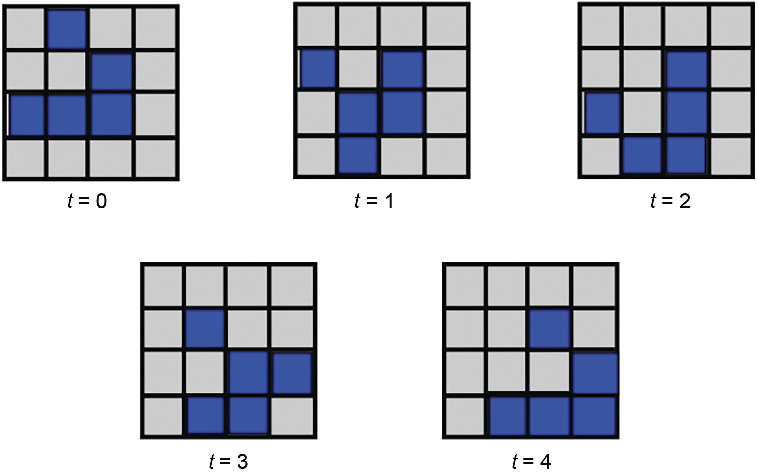
\includegraphics{graphics/Chapter_02/Figure1.pdf}}{Scheme of the translation of the ``Hello world!'' program from assembly code to hexadecimal code.}[-350pt,3pt]\vspace*{9pt}
\caption{\label{fig:2.1}The assembly instructions and the machine code of a very simple program that prints the string ``Hello world!'' An assembler program must be used to translate the original instruction to machine operations (here represented in a hexadecimal format).}
\end{figure}

Approximately ten years after the first production and use of digital \hbox{computers,} it was usual to implement software programs using assembly languages to avoid the hard-coding, error-prone, tedious, and time-consuming first-generation machine language programming used with the earliest computers, freeing programmers from keeping track of binary codes and data addresses. From a historical viewpoint, Kathleen Booth is recognized as the inventor of the first assembly language in 1947. In late 1948, David Wheeler developed the first assembler program for the EDSAC and integrated it into the computer bootstrap program. For around another ten years algorithms in digital computers were coded using assembly languages. However, by the late 1950s the use of assembly languages had been replaced by the so-called high-level languages---with the goal of improving programming productivity and guarantying portability of algorithms from one computer to another with a different CPU. Today, assembly languages are still used for direct hardware manipulation in modes unsupported by a higher-level language, programming specific embedded hardware systems, accessing specialized processor instructions, or solving critical performance issues. For example, in operating systems development, where from the early 1950s to the end of the 1960s most operating systems were entirely implemented using assembly languages, today only 1\% to 2\% of the operating system kernel code is written in assembly; the rest, that is, more than 98\%, is written in high-level languages such as C, C++, and Java.




It is worth mentioning that the assembly language of the \textit{Apollo Guidance\break Computer} (AGC) produced for the Apollo program and installed on board each Apollo command module and Apollo Lunar Module was the first programming language to land on the Moon. On July 20, 1969, the algorithms that managed and steered Apollo 11 landed on the Moon on board the Eagle lunar module together with Neil Armstrong and Buzz Aldrin. The software of the AGC contained about 145,000 lines of code and was implemented by a team of 350 programmers headed by Margaret Hamilton. She was the director of the Software Engineering Division of the MIT Instrumentation Laboratory, where the software for NASA's Apollo program was developed. Despite its complexity and very long list of instructions, bugs were never known to have occurred during any Apollo mission.

\section{\label{sec:2.5}High-level Languages, Concepts, and Evolution}

A simple way to classify programming languages is to divide them between low-level and high-level languages. Low-level programming languages provide little or no abstraction from a computer's instruction set architecture. Their instructions are very simple and hard to read (for humans). Machine languages and assembly languages belong to this class. Low-level languages can be considered as being close to the hardware operations and far away from human languages. Programs written in low-level programming languages do not provide a good abstraction from hardware and are generally non-portable from one system's architecture to another. Conversely, high-level programming languages provide abstraction from the details of the computer hardware and offer a way to express algorithms in a style similar to human languages. In fact, they use human language names, lexicons, and syntax, making the process of programming an algorithm easier, faster, and more readable than when a lower-level programming language is used. Different high-level languages provide diverse levels of abstraction that allow a programmer to be detached from the machine hardware details. The use of high-level languages in coding algorithms often results in lower performance because each high-level instruction must be translated (by a compiler or an interpreter) to a sequence of machine language instructions. However, the benefits in terms of productivity, portability, modifiability, and readability are so significant that they are the most used languages today.

A compiler is a program designed to translate code written in one high-level programming language (the ``source language'') into another language (the \hbox{``target} language''), typically low level (e.g., assembly language or machine code), to create an executable program that can be executed by a given CPU or a class of CPUs sharing hardware features. Among the main tasks of a compiler is to control the correctness of the source code through lexical, syntax, and semantic analysis and the production of the executable code. By contrast, an interpreter is a software program that analyzes each single instruction of a program (generally coded in a high-level language) and directly executes it without requiring it to previously have been compiled into a machine language program. If an instruction is incorrect, the interpreter stops the program execution, and the next instructions will not be executed. An interpreter generally uses different strategies for program execution as follows:

\begin{itemize}
\item Sequentially analyze the program source code and execute its instructions directly.

\item Translate code into an intermediate representation (or object code) and immediately execute that.
\end{itemize}

\noindent An interpreter can sometimes be used together with a compiler: for example, when pre-compiled intermediate code (i.e., bytecode) produced by a compiler is passed to an interpreter to be executed. In this case, the interpreter is able to read each bytecode instruction and execute it.

While programs were developed in machine or assembly languages in the first few decades of the computer age, today most software applications are implemented in high-level interpreted and/or compiled languages. The first commonly used high-level programming language was FORTRAN (FORmula TRANslator), a language designed in 1957 by a team led by John Backus at IBM. The FORTRAN language was developed for programming scientific, mathematical, and statistical algorithms, and, after more than 70 years and several extended versions, it is still in use today for programming and executing scientific applications. Before IBM developed the FORTRAN language, other high-level languages such as Plankalk\"{u}l (Plan Calculus), Short Code, and Autocode were designed and partially implemented, although they were not used by many programmers. Examples of  statements defined in FORTRAN and in the early high-level programming languages are the \texttt{IF} conditional statement, the \texttt{READ} and \texttt{WRITE} statements for input/{\allowbreak}output operations, the \texttt{GO~TO} jump unconditional statement, and the \texttt{DO} loop for executing a group of operations until a given condition becomes false. The use of these high-level statements improved the productivity of programmers in software implementation, simplified their programming tasks, and made the program code much more concise and easier to read. Two or three years after FORTRAN was introduced, other high-level languages such as ALGOL (Algorithmic Language), LISP (List Processor), and COBOL (Common Business-Oriented Language) were developed. In particular, the programming model used in ALGOL served as the basis for the development of some of the most important high-level programming languages including Simula, Pascal, C, C++, and Java.

In 1964, a team of students at Dartmouth College developed the BASIC \hbox{(Beginner's} All-Purpose Symbolic Instruction Code) language that ten years later was developed further by Bill Gates and Paul Allen and became the first marketable product of Microsoft. While BASIC used very simple programming instructions and structures that made it very easy to learn and use, not many checks were carried out by the compiler on its data abstractions and operations. As the years passed, several new programming languages were developed that allowed faster and more efficient production of software. In 1970, Niklaus Wirth developed \hbox{PASCAL,} a very well-structured programming language in honor of the French mathematician Blaise Pascal. In 1972 at Xerox Labs, Alan Key and his team implemented the Smalltalk language that introduced a set of programming concepts and mechanisms that are used today in languages such as Python, Java, and Ruby. Smalltalk was the first object-oriented language, that is, a language based on the concept of ``objects,'' which contain data (with their attributes) and code in the form of procedures (or methods). A common feature of objects is that methods are associated to them and only methods can be used to read and modify the object's data fields. This feature allows a more abstract way to implement software programs and verify their correctness. In the same year, Dennis Ritchie at Bell Telephone Laboratories worked on a new programming language for coding application and system programs and developed the C language. After implementing a compiler, together with Ken Thompson he used the language to implement the Unix operating system. The new language was called C simply because it was based on an earlier language called B. Some current leading languages such as C++, C\#, Java, JavaScript, Perl, PHP, and Python are in part derivatives of~C. 

\section{\label{sec:2.6}Source and Executable Code}

The collection of high-level programming languages is extensive and cannot be completely listed here. However, some other modern languages are Ada, Objective-C, Perl, Haskell, Visual Basic, JavaScript, Python, PHP, Ruby, Scala, Swift, and Go. For a quick and simple comparison of low-level languages, such as machine and assembly languages, with high-level languages, Figure~\ref{fig:2.2} shows the program code written in C language of the trivial ``Hello world!'' program that was introduced in Figure~\ref{fig:2.1}. In contrast to assembly statements that require deep programming skills, the very few statements of this C program can be read by non-specialists. In particular, after the \texttt{\#include} directive that is used to include in the program the input/{\allowbreak}output standard library---for allowing the printing of strings of text on the screen---and the \texttt{main()} statement that starts the operations, the C program uses only one statement (the \texttt{printf} function), whereas the machine and assembly programs in Figure~\ref{fig:2.1} use more than ten instructions to code this very trivial program.

\begin{figure}[!t]
\begin{tabular}{l}
\texttt{\#include <stdio.h>}\\
\texttt{main ()}\\
\texttt{\{}\\
\texttt{printf(``Hello World!'');}\\
\texttt{\}}
\end{tabular}
\caption{\label{fig:2.2}The C code of a program that prints the string ``Hello world!'' A C compiler is used to translate this program to machine instructions that will be executed by the language runtime.}
\end{figure}

To show how a high-level language allows programmers to code algorithms, we describe the C code of two algorithms introduced in Chapter~\ExternalLink{chap:1}{1}. The first one, shown in Figure~\ref{fig:2.3}, is the Euclid algorithm that finds the greatest common divisor of two positive integers \textit{a} and \textit{b}. The greatest common divisor of two numbers is the largest number that divides both. A simple method to find that divisor is to factorize both numbers and multiply common factors.


\begin{figure}[!b]
\begin{tabular}{l}
\texttt{\#include <stdio.h>}\\
\texttt{main ()}\\
\texttt{\{}\\
\texttt{int a, b, r;}\\
\texttt{scanf(``Insert the first value \%d'', \&a);}\\
\texttt{scanf(``Insert the second value \%d'', \&b);}\\
\texttt{while (b>0) \{}\\
\quad\texttt{r=a\%b;}\\
\quad\texttt{a=b;}\\
\quad\texttt{b=r;}\\
\texttt{\}}\\
\texttt{printf(``GCD is: ''a);}\\
\texttt{\}}
\end{tabular}
\caption{\label{fig:2.3}The C code of the Euclid algorithm that finds the greatest common divisor of two positive integers.}
\end{figure}


Let us use integer variables \textit{a} and \textit{b} to represent the two numbers and the variable \textit{r} to represent the remainder of their division, that is, \textit{r} is equal to \textit{a \% b}. After reading the two values by using the \texttt{scanf }function, the \texttt{while} loop is utilized to determine the remainder \textit{r} and assign current values of variables \textit{b} and \textit{r} to variables \textit{a} and \textit{b}, respectively. Please note that the symbol ``$=$'' used in the three operations into the while loop is the assignment operator used in C and in other languages to assign a value to a variable. The assignment operator is different from the equality operator that is expressed by a double equal sign ``${=}{=}$'' (see the program in Figure~\ref{fig:2.4}). Execution of the operations in the \texttt{while} loop is continued as long as the value of divisor \textit{b} is greater than zero. When the value of \textit{b} becomes zero, the value of variable \textit{a} is the GCD of the given numbers, and it is visualized by the \texttt{printf} statement.

In Chapter \ExternalLink{chap:1}{1}, we also introduced the simple linear search algorithm for finding a given value in a list of numbers. Here (see Figure~\ref{fig:2.4}), we show the C program that implements that algorithm. After reading the list of elements through the \texttt{for} loop, the program asks for the number to be searched \texttt{(scanf(``\%d'', \&x);)}, and then sequentially through the second \texttt{for} loop compares each element $S[i]$ with the element to search \textit{x} until it finds it and prints its position or the list ends, in this case the program signals that the number is not present in the list.

\begin{figure}[!b]
\begin{tabular}{l}
\texttt{\#include <stdio.h>}\\
\texttt{main ()}\\
\texttt{\{}\\
\texttt{int N = 100, S[N], x, i, j;}\\
\texttt{printf(``Enter \%d integers: '');}\\
\texttt{for (i = 0; i < N; i++)}\\
\qquad\texttt{scanf(``\%d'', \&S[i]);}\\
\texttt{printf(``Enter a number to search: '');}\\
\texttt{scanf(``\%d'', \&x);}\\
\texttt{for (i = 0; i < N; i++)\{}\\
\quad\texttt{if (S[i] == X) \{}\\
\qquad\texttt{printf(``\%d is at location \%d.'', x, i+1);}\\
\qquad\texttt{break;}\\
\quad\texttt{\}}\\
\texttt{\}}\\
\texttt{if (i == N)}\\
\quad\texttt{printf(``\%d is not present in the list \%d.'', x);}\\
\texttt{\}}
\end{tabular}
\caption{\label{fig:2.4}The C program implementing the linear search algorithm that, given an array of elements of size $N=100$, let find a given value \textit{x}, if it is within the array.}
\end{figure}


Although the C source code requires a few technical commands to be included (for instance, the \texttt{\#include} directive, the parentheses for grouping blocks of code, and some data format pragma such as \texttt{\%d}), the program is readable and understandable enough for non-experts. Source code in high-level languages is in fact a sequence of human-readable instructions that programmers write when they develop the program. Program code is then stored in files for further changes or for producing executable code by a compiler. When the source code is complete, it is run through a compiler to turn it into machine code called executable code. This is a program code that a computer can understand and execute but humans are no longer able to read and change appropriately because machine code consists of binary sequences of 1s and 0s that are not human-readable. While most high-level programming languages use a compiler-based approach to produce machine code, a few programming languages, such as JavaScript or PHP, are interpreted instead. In interpreted languages, the distinction between source code and executable code does not apply because there is only the source code that is analyzed and executed by an interpreter that processes each single instruction and, if correct, generates the corresponding machine code to be executed. Generally, application software is distributed in a form that includes only executable files. This means that we can install and run that software but we cannot modify or reuse it in other programs. If the source code of programs is included, it would be useful to a programmer or a systems developer who might wish to study and/or modify that code.

In this context, the concept of \textit{open-source} programs plays an important role. This term was coined in the field of software development to describe a specific approach to building and distributing computer programs. Today, however, the keyword ``open source'' describes a broader set of values, projects, products, and initiatives that include and celebrate principles of open exchange, collaborative participation, rapid prototyping, transparency, and community-oriented development. The open-source model is a decentralized software development and \hbox{maintenance} standard that encourage open collaboration among software programmers, teams, and companies. A main principle of open-source software development is peer production, with products such as source code, schemes, and documentation freely available to the public. According to this approach, the source code of programs is distributed together with the executable to allow users and programmers to learn the algorithms used in these software programs and modify/{\allowbreak}extend them if needed.

Open-source technology benefits both expert programmers and end-users. In fact, computer users prefer open-source software to proprietary software for several practical reasons, including control of the used algorithms, security in execution, readability, and training. Some open-source licenses require that anyone who releases a modified open-source program must also release the source code for that program. Furthermore, we must keep in mind that some licenses specify that who ever alters and shares an open-source program with others must also share that program's source code without charging a licensing fee for it.


\section{\label{sec:2.7}Software Applications}

The number of software applications that are used today in every moment and every aspect of our daily life is immeasurable. For every action we take at work or at home there is an application that may assist us. We can say that the relationship of human beings with reality is more and more often and more deeply regulated by algorithms, which encode billions of operations that are recorded in digital storage and executed by the CPUs of computers, smartphones, webcams, sensors, smartwatches, and many other digital devices. Application software, also known as end-user software or productivity software, include algorithms that perform specific personal, educational, and business functions. Each application is designed to assist end-users in accomplishing a variety of tasks, which can be linked to data processing, productivity, communication, traveling, or creativity. The most common software application platforms today are used by millions of people every day. Applications like Spotify, Chrome, Firefox, Zoom, Gmail, Word, and many others are designed to help with specific tasks that are increasingly vital for people.

The functions implemented by application software can be personal, business, as well as educational. Each software program is developed by using high-level programming languages to assist people with a particular process related to productivity, efficiency, or communication. The large number of apps that are installed on our smartphones are clear examples of application software. For over 6.5 billion smartphone users across the world, software apps have become their everyday companion and most software apps are becoming irreplaceable for many of us. As Statista (\href{https://www.statista.com}{www.statista.com}) reported, in the first quarter of 2021, ``Android users were able to choose between 3.48 million apps, making Google Play the app store with biggest number of available apps. The Apple App Store was the second-largest app store with roughly 2.22 million available apps for iOS.'' The average price of an app in the App Store amounts to US\$0.91. Other than Apple and Google, who dominate the app market, there are a few other players such as Amazon Appstore, offering about 500,000 Android apps to worldwide audiences, and the Tencent Appstore, with around 50,000 available apps as of 2022. This impressive scenario makes evident the very important role of algorithms, which through the exploitation of programming languages can be implemented as software programs and run very fast on billions of digital devices.


\begin{thebibliography}{}

\bibitem[Boole(1848)]{chap:02:Boole:1848} G. Boole. 1848. The calculus of logic. \textit{Camb. Dublin Math. J.} 3, 183--198.

\bibitem[Boole(2009)]{chap:02:Boole:2009}G. Boole. 2009. \textit{An Investigation of the Laws of Thought on Which Are Founded the Mathematical Theories of Logic and Probabilities}. Cambridge University Press, Cambridge.

\bibitem[Davis(2012)]{chap:02:Davis:2012} M. Davis. 2012. \textit{The Universal Computer: The Road from Leibniz to Turing}. CRC Press.

\bibitem[G\"{o}del(1931)]{chap:02:Godel:1931} K. G\"{o}del. 1931. \"{U}ber formal unentscheidbare S\"{a}tze der Principia Mathematica und verwandter Systeme I. \textit{Monatshefte f\"{u}r Mathematik und Physik} 38, 1, 173--198. DOI:~\href{https://doi.org/10.1007/BF01700692}{https://{\allowbreak}doi.{\allowbreak}org/{\allowbreak}10.{\allowbreak}1007/{\allowbreak}BF01700692}.

\bibitem[Neumann(1945)]{chap:02:Neumann:1945} J. v. Neumann. June 1945. \textit{First Draft of a Report on the EDVAC}. Moore School of Electrical Engineering, University of Pennsylvania.

\bibitem[Shannon's(1938)]{chap:02:Shannon:1938} C. E. Shannon. 1938. A symbolic analysis of relay and switching circuits. \textit{Trans. Am. Inst. Electr. Eng.} 57, 713--723. DOI:~\href{http://doi.org/10.1109/T-AIEE.1938.5057767}{http://{\allowbreak}doi.{\allowbreak}org/{\allowbreak}10.{\allowbreak}1109/{\allowbreak}T-{\allowbreak}AIEE.{\allowbreak}1938.{\allowbreak}5057767}.

\bibitem[Smith(2014)]{chap:02:Smith:2014} J. T. Smith. 2014. David Hilbert's radio address---German and English. Mathematical Association of America. [Online]. Retrieved June 10, 2022 from \href{https://www.maa.org/press/periodicals/convergence/david-hilberts-radio-address-german-and-english}{https://{\allowbreak}www.{\allowbreak}maa.{\allowbreak}org/{\allowbreak}press/{\allowbreak}periodicals/{\allowbreak}convergence/{\allowbreak}david-hilberts-{\allowbreak}radio-{\allowbreak}address-{\allowbreak}german-{\allowbreak}and-english}.

\bibitem[Turing(1937)]{chap:02:Turing:1937} A. M. Turing. 1937. On computable numbers, with an application to the Entscheidungsproblem. \textit{Proc. London Math. Soc.} s2--42, 1, 230--265. DOI:~\href{https://doi.org/10.1112/plms/s2-42.1.230}{https://{\allowbreak}doi.{\allowbreak}org/{\allowbreak}10.{\allowbreak}1112/{\allowbreak}plms/{\allowbreak}s2-{\allowbreak}42.{\allowbreak}1.230}.
\end{thebibliography}

%\end{document}

